%%This is a very basic article template.
%%There is just one section and two subsections.
\documentclass{article}
\usepackage{amsmath}
\usepackage{pgf}
\usepackage{lastpage}
\usepackage{amssymb}
\usepackage{tikz}
\usepackage[margin=0.75in]{geometry}
\usetikzlibrary{arrows,matrix,positioning}
\usepackage{listings}             % Include the  listings-package
\usepackage[utf8]{inputenc}
\usepackage[english]{babel}
\usepackage{fancyhdr}
 
\lstset{language=Matlab} 
\pagestyle{fancy}
\fancyhf{}
\fancyhead[LE,RO]{Homework 3 - Greg Timmons}
\fancyhead[RE,LO]{CSC 579 - Perf Modeling}
\fancypagestyle{plain}{
\fancyfoot[LE,RO]{\thepage\backslash\pageref{LastPage}}  
} 
\fancyfoot[LE,RO]{\thepage\backslash\pageref{LastPage}}  
\usetikzlibrary{arrows,automata}
\usepackage[latin1]{inputenc}
\usepackage{pdfpages}



\begin{document}
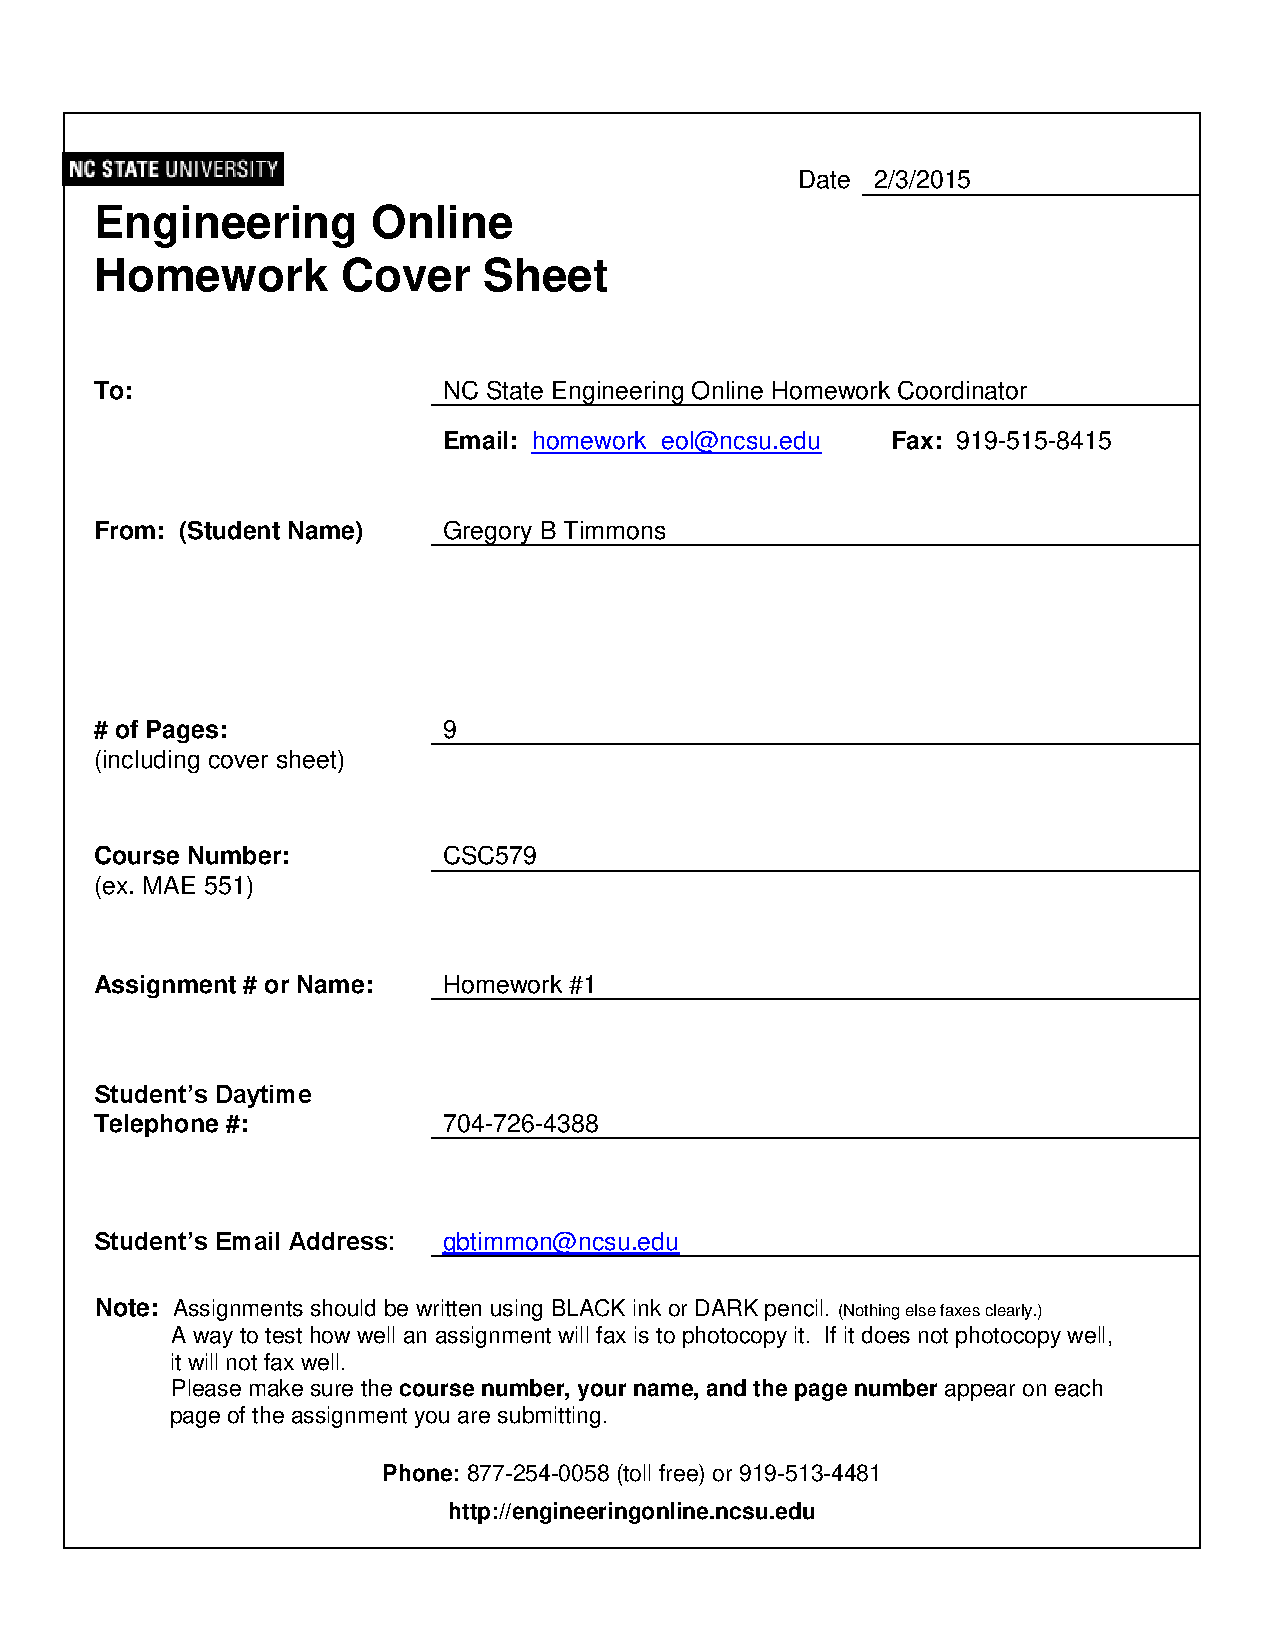
\includepdf[pages={1}]{cover.pdf}
\title{Homework 3}
\date{March 22, 2015}
\author{Gregory B Timmons, gbtimmon}
\maketitle
\section*{Question 1}
\[ P = 
\left(\begin{array}{ccccc}
0.2   & 0.0   & 0.005 & 0.795 & 0.0   \\
0.0   & 0.0   & 0.998 & 0.002 & 0.0   \\
0.002 & 0.0   & 0.0   & 0.0   & 0.998 \\
0.8   & 0.001 & 0.0   & 0.198 & 0.001 \\
0.0   & 0.998 & 0.0   & 0.002 & 0.0   
\end{array}\right)
\]
\\	
\[ P_{HB} = \]\[
\begin{array}{ccccccccccccc}
0.2 &0.005 &0.795 &0.998 &0.002 &0.002 &0.998 &0.8 &0.001 &0.198 &0.001 &0.998 &0.002 \\
1 &3 &4 &3 &4 &1 &5 &1 &2 &4 &5 &2 &4 \\
1 &4 &6 &8 &12 &14 
\end{array}
\]

\[ Q_{HB} = (P^{T} - I)^{T}_{HB} = \]\[
\begin{array}{cccccccccccccccc}
-0.8 &0.005 &0.795 &-1 &0.998 &0.002 &0.002 &-1 &0.998 &0.8 &0.001 &-0.802
&0.001 &0.998 &0.002 &-1 \\
1 &3 &4 &2 &3 &4 &1 &3 &5 &1 &2 &4 &5 &2 &4 &5 \\
1 &4 &7 &10 &14 &17 
\end{array}\]
\section*{Question 2}
The Gauss-Siedel was computed on the Harwell Boeing matrix using the following
matlab code 
\begin{lstlisting}[frame=single] 
 function pi = HW3_gaussSeidel(pi, V, J, I)
    for s = 2 : size(I, 2)  
        sum = 0;
        for i = I(s-1):I(s)-1
            sum = sum + pi(J(i))*V(i);
        end  
        pi(s-1) = sum;
    end
end 
\end{lstlisting}
Using the values \\
$ V = \left(\begin{array}{ccccccc}
	0.4 & 0.6 & 0.4 & 0.4 & 0.2 & 0.2 & 0.8 \\
\end{array}\right)$\\
$ J    = \left(\begin{array}{ccccccc}
	3 & 1 & 2 & 1 & 3 & 3 & 2 \\
\end{array}\right)$\\
$ I   = \left(\begin{array}{cccc}
	1 & 3 & 6 & 8 \\
\end{array}\right)$\\
\\
with \\
$\pi^{(0)} = \left(\begin{array}{ccc}
	0 & 1 & 0
\end{array}\right)$ \\ 
\\
I computed the following values :\\
$\pi^{(1)} = \left(\begin{array}{ccc}
	0  &  0.5556  &  0.4444
\end{array}\right)$ \\ 
$\pi^{(2)} = \left(\begin{array}{ccc}
0.3135   & 0.3407  &  0.3459
\end{array}\right)$ \\ 

\section*{Question 3}
Interarrival time $1/\lambda = .25$ -- mean arrival rate
$\lambda = 4$ \subsection*{(a)}
\[ p_{0}(.5) = e^{-(.5)} = 0.135 \]
\subsection*{(b)}
At a rate of 4 per hours, we expect to reach ten customers at 2.5 hours. 
\sub
\end{document}
